我们在\autoref{prop:1.3}中已经看到，赋予 $W_2$ 距离的 $\mathcal P_2(\mathbb R^d)$ 具有度量空间结构. 实际上，它的几何结构丰富得多，因为它类似于一个黎曼流形（Riemannian manifold）. 因此，可以将黎曼几何的计算法则——在这里称为 Otto 微积分（Otto calculus）——用于概率测度空间上算法的设计与解释.

将 $\mathcal P_2(\mathbb R^d)$ 视为黎曼流形纯粹是“形式的”，即启发式的. 例如，$\mathcal P_2(\mathbb R^d)$ 并不局部同胚于 Hilbert 空间. 不过，这一黎曼视角仍是理解 Wasserstein 空间几何性质的有力工具.

为阐明这一视角，本章使用绝对连续测度；对于它们，可以为黎曼形式体系建立更严格的基础. 构造这一体系的主要目标，是在 Wasserstein 空间上定义由梯度流给出的有意义的动力学. 定义这些动力学后，我们将看到，即使对于非绝对连续测度，它们也常常有意义；特别地，它们为被视作粒子系统的离散测度给出良定义的动力学. 一旦推导出来，就可以直接研究离散测度上的这些非平凡动力学，而不必严格解释离散情形中的黎曼计算. 希望了解一般测度梯度流的完全严格推导的读者，可以查阅 Ambrosio 等人的奠基性专著\cite{ref18}，或阅读\cite{ref282}中的简要综述.

\subsection{度量导数与连续性方程}\label{sec:5.1}

最优传输的作用在于，为概率测度空间赋予一种尊重底层空间几何的几何结构. 例如，我们已经看到，映射 $x\mapsto\delta_x$ 将 $(\mathbb R^d,\|\cdot\|)$ 等距嵌入 $(\mathcal P_2(\mathbb R^d),W_2)$. 因此，现在研究 $\mathcal P_2(\mathbb R^d)$ 上的动力学时，我们的方法是“提升”$\mathbb R^d$ 中相应的粒子动力学.

使用微分学规定 $\mathbb R^d$ 上动力学的一般方式是常微分方程（ordinary differential equation，ODE）. 具体而言，给定依赖时间的向量场族 $(v_t)_{t\geq0}$，考虑 ODE
\begin{equation}\label{eq:5.1}
\dot X_t=v_t(X_t).
\end{equation}
在对 $(v_t)_{t\geq0}$ 的标准假设下，\footnote{例如，若向量场关于时间一致地满足 Lipschitz 条件，则由 Cauchy--Lipschitz 定理得到适定性.}对任意给定的初值 $X_0$，这一 ODE 都存在唯一解. 现在假设初值 $X_0$ 是从某个测度 $\mu_0\in\mathcal P_2(\mathbb R^d)$ 中随机抽取的；类似地，对所有 $t\geq0$，用 $\mu_t$ 表示 $X_t$ 的分布. 可以将测度曲线 $(\mu_t)_{t\geq0}$ 看成一群粒子的演化. 那么，$(\mu_t)_{t\geq0}$ 的动力学由一个称为连续性方程（continuity equation）的偏微分方程（partial differential equation，PDE）描述.

\begin{proposition}[连续性方程]\label{prop:5.1}
假设 $X_0\sim\mu_0$，且 $(X_t)_{t\geq0}$ 按照\eqref{eq:5.1}演化，并假设该动力学适定. 对所有 $t\geq0$，用 $\mu_t$ 表示 $X_t$ 的分布. 那么 $(\mu_t)_{t\geq0}$ 在弱意义下满足
\begin{equation}\label{eq:5.2}\index{continuity equation@连续性方程（continuity equation）|hyperpage}
\partial_t\mu_t+\operatorname{div}(\mu_tv_t)=0,
\end{equation}
即对于任意紧支撑光滑检验函数 $\varphi:\mathbb R^d\to\mathbb R$，有
\begin{equation}\label{eq:5.3}
\partial_t\int\varphi\,d\mu_t=\int\langle\nabla\varphi,v_t\rangle\,d\mu_t.
\end{equation}
\end{proposition}

用概率语言写出\eqref{eq:5.3}，即为 $\partial_t\mathbb E\varphi(X_t)=\mathbb E\langle\nabla\varphi(X_t),v_t(X_t)\rangle$，它直接由\eqref{eq:5.1}和链式法则得到. 这一命题真正的内容在\eqref{eq:5.2}：若 $\mu_t$ 关于 Lebesgue 测度具有光滑密度，并滥用记号仍用 $\mu_t$ 表示该密度，则分部积分给出
$$
\begin{aligned}
\int\varphi\,\partial_t\mu_t
&=\partial_t\int\varphi\,d\mu_t
=\int\langle\nabla\varphi,v_t\rangle\mu_t\\
&=-\int\varphi\operatorname{div}(\mu_tv_t).
\end{aligned}
$$
因为这一等式对所有合适的检验函数 $\varphi$ 都成立，所以\eqref{eq:5.2}逐点成立. 因此，至少当 $\mu_t$ 在所有 $t\geq0$ 都有光滑密度时，$(\mu_t)_{t\geq0}$ 解 PDE \eqref{eq:5.2}. 一般而言，在预先不知道 $\mu_t$ 正则性的情况下，陈述适用于曲线 $(\mu_t)_{t\geq0}$ 的结果更为方便；这时应将\eqref{eq:5.2}解释为弱意义的\eqref{eq:5.3}. 不过，为使 Otto 微积分框架的发展不受技术细节干扰，以下忽略这些正则性问题，并假定我们使用的都是光滑密度曲线. 更严格的处理见\cite{ref18}.

\eqref{eq:5.1}与\eqref{eq:5.2}为同一动力学提供了两种对偶视角；在流体力学中，它们分别称为 Lagrange 视角与 Euler 视角. Lagrange 视角描述单个粒子轨迹的演化，而 Euler 视角通过质量密度 $\mu_t$ 与速度场 $v_t$，追踪整体量的演化.

为预示 $\mathcal P_2(\mathbb R^d)$ 上的几何构造，先考察如何在 $\mathbb R^d$ 上建立几何；暂且宽泛地使用黎曼几何概念，并在\autoref{sec:5.2}回到这一主题. 对按照\eqref{eq:5.1}演化的单个粒子轨迹 $t\mapsto X_t$，假设粒子质量为一，则其在时刻 $t$ 的动能为 $\|\dot X_t\|^2=\|v_t(X_t)\|^2$. 曲线在时间区间 $[0,1]$ 上的总能量为 $\int_0^1\|v_t(X_t)\|^2\,dt$；在所有满足\eqref{eq:5.1}、且端点固定为 $X_0$ 和 $X_1$ 的曲线 $(X_t)_{t\in[0,1]}$ 上最小化该能量，得到常速测地线 $t\mapsto X_t:=(1-t)X_0+tX_1$. 从几何上看，$v_t(X_t)$ 是曲线在时刻 $t$ 的切向量，其长度由欧氏范数 $\|\cdot\|$ 衡量.

现在尝试将这幅图景提升至 $\mathcal P_2(\mathbb R^d)$. 对按照\eqref{eq:5.2}演化的曲线 $(\mu_t)_{t\geq0}$，自然可以把速度向量场 $v_t:\mathbb R^d\to\mathbb R^d$ 看成曲线在时刻 $t$ 的抽象“切向量”，并通过动能衡量其“长度”的平方：\footnote{因为 $\mu_t$ 起质量密度的作用，$\|v_t\|^2\mu_t$ 就是动能密度，在全空间积分得到动能.}
\begin{equation}\label{eq:5.4}
\|v_t\|_{\mu_t}^2:=\int\|v_t\|^2\,d\mu_t.
\end{equation}
但这样做立即遇到障碍：给定曲线 $(\mu_t)_{t\geq0}$，使\eqref{eq:5.2}成立的向量场族 $(v_t)_{t\geq0}$ 不唯一，因此不清楚应选择哪个 $v_t$ 作为切向量. 的确，若从任何满足\eqref{eq:5.2}的向量场族出发，且 $w_t$ 对所有 $t\geq0$ 满足 $\operatorname{div}(\mu_tw_t)=0$，则由散度算子的线性性，$(v_t+w_t)_{t\geq0}$ 也是满足\eqref{eq:5.2}的一族向量场. 一个具体的非唯一性例子是：设 $\mu_t$ 对所有 $t\geq0$ 都是 $\mathbb R^2$ 上的标准高斯分布. 一种自然选择是始终取 $v_t=0$；但由于标准高斯分布的旋转不变性，另一种选择是取产生旋转的向量场（见\autoref{fig:5.1}）.

\autoref{fig:5.1}右侧的向量场给粒子引入了多余运动，因此并非对 $(\mu_t)_{t\geq0}$ 动力学的最简洁解释. 为消除向量场选择的歧义，我们可以规定：在仍能解释测度曲线动力学的前提下，选取使动能\eqref{eq:5.4}最小的向量场作为切向量. 如下所述，动能最小化也自然契合质量“最优”传输的思想.

\begin{figure}[htbp]
\centering
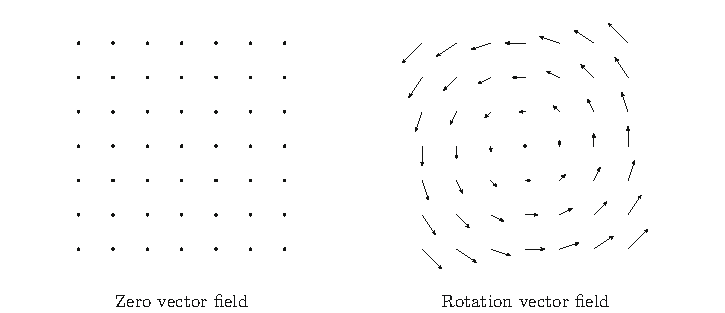
\includegraphics[width=0.92\linewidth]{assets/chapter5/fig5-1.pdf}
\caption{两种保持 $\mathbb R^2$ 上标准高斯分布的向量场：左为零向量场，右为旋转向量场.}\label{fig:5.1}
\end{figure}

为进一步说明这一选择的动机，引入度量空间 $(S,\mathsf d)$ 中曲线 $(x_t)_{t\geq0}$ 的度量导数（metric derivative）. 虽然一般无法赋予一般度量空间中曲线的切向量或“导数”以意义，却可以赋予其速度以意义.

\begin{definition}[度量导数]\label{def:5.2}\index{metric derivative@度量导数（metric derivative）|hyperpage}
设 $(S,\mathsf d)$ 为度量空间，$(x_t)_{t\geq0}$ 为 $S$ 中曲线. 若下列极限存在，则曲线在时刻 $t$ 的度量导数为
$$
|\dot x|(t):=\lim_{s\to t,\ s\ne t}\frac{\mathsf d(x_s,x_t)}{|s-t|}.
$$
\end{definition}

下一个定理表明，这一选择原则产生了良定义的切向量 $v_t$，它有三种刻画方式：(1) 在约束\eqref{eq:5.2}下动能最小的向量场；(2) 满足\eqref{eq:5.2}、且长度 $\|v_t\|_{\mu_t}$ 等于度量导数 $|\dot\mu|(t)$ 的唯一向量场；(3) Brenier 映射的极限.

不过，先引入与 ODE \eqref{eq:5.1}（等价地，与向量场族 $(v_t)_{t\geq0}$）关联的流映射（flow map）. 映射 $F_{0,t}:\mathbb R^d\to\mathbb R^d$ 将给定的 $X_0$ 映为从 $X_0$ 出发的 ODE 在时刻 $t$ 的解 $X_t$. 类似地，对任意两个时刻 $0\leq s\leq t$，可以定义 $F_{s,t}:\mathbb R^d\to\mathbb R^d$. 这个定义的意义在于，将注意力从 ODE 所描述的一条轨迹转向整个空间 $\mathbb R^d$ 在 ODE 作用下的形变.

给定 $\mu,\nu\in\mathcal P_2(\mathbb R^d)$，其中 $\mu$ 有密度，用 $T_{\mu\to\nu}$ 表示从 $\mu$ 到 $\nu$ 的 Brenier 映射，并用 $|\dot\mu|$ 表示 $\mathcal P_2(\mathbb R^d)$ 中曲线相对于度量 $\mathsf d=W_2$ 的度量导数.

\begin{theorem}\label{thm:5.3}
设 $(\mu_t)_{t\geq0}$ 为一条正则的\footnote{这里“正则”可理解为 $\mu_t\in\mathcal P_2(\mathbb R^d)$ 且有密度，并且 $|\dot\mu|(t)$ 对所有 $t\geq0$ 存在. 假设与结论中的“对所有 $t\geq0$”可以替换为“对几乎所有 $t\geq0$”，有密度的假设也可以放宽.}概率测度曲线. 那么，对于满足\eqref{eq:5.2}的每一向量场族 $(v_t)_{t\geq0}$，所有 $t\geq0$ 都有 $|\dot\mu|(t)\leq\|v_t\|_{\mu_t}$.

反之，存在唯一的族 $(v_t)_{t\geq0}$ 满足\eqref{eq:5.2}，并且对每个 $t\geq0$ 有 $|\dot\mu|(t)=\|v_t\|_{\mu_t}$. 这一族满足
\begin{equation}\label{eq:5.5}
v_t=\lim_{h\searrow0}\frac{T_{\mu_t\to\mu_{t+h}}-\mathrm{id}}{h}
\qquad\text{在 }L^2(\mu_t)\text{ 中},
\end{equation}
其中 $\mathrm{id}$ 为恒等函数.
\end{theorem}
\begin{proof}[证明草图]
先证明第一个结论. 设 $(X_t)_{t\geq0}$ 为求解 $\dot X_t=v_t(X_t)$ 的随机变量曲线，且 $X_0\sim\mu_0$. 因为假设连续性方程\eqref{eq:5.2}成立，所以对所有 $t\geq0$ 有 $X_t\sim\mu_t$；特别地，$\mu_{t+h}=(F_{t,t+h})_\#\mu_t$. 利用这个次优耦合可以得到 $W_2(\mu_t,\mu_{t+h})$ 的上界：
$$
\frac{W_2^2(\mu_t,\mu_{t+h})}{h^2}
\leq\mathbb E\left[\frac{\|F_{t,t+h}(X_t)-X_t\|^2}{h^2}\right].
$$
注意 $F_{t,t+h}(X_t)=X_t+hv_t(X_t)+o(h)$，令 $h\to0$，得到 $|\dot\mu|(t)\leq\sqrt{\mathbb E[\|v_t(X_t)\|^2]}=\|v_t\|_{\mu_t}$.

上面的不等式来自采用次优耦合. 直观上，若使 $X_t$ 和 $X_{t+h}$ 最优耦合，并由\eqref{eq:5.5}定义 $v_t$，应当得到等式. 的确如此，但这里省略证明.

最后，结合两项结论可知，若 $(v_t)_{t\geq0}$ 满足\eqref{eq:5.2}且 $|\dot\mu|(t)=\|v_t\|_{\mu_t}$，则
$$
0\in\operatorname*{arg\,min}_{w_t:\mathbb R^d\to\mathbb R^d}\|v_t+w_t\|_{\mu_t}
\quad\text{满足}\quad\operatorname{div}(\mu_tw_t)=0.
$$
而且这是严格凸问题，所以极小化解唯一. 因此，若 $(v_t)_{t\geq0}$ 与 $(u_t)_{t\geq0}$ 均满足连续性方程，且 $\|v_t\|_{\mu_t}=\|u_t\|_{\mu_t}=|\dot\mu|(t)$，则 $w_t=u_t-v_t=0$，得到所述结论.
\end{proof}

上一定理在写出\eqref{eq:5.5}、即断言最优传输映射存在时，使用了 $\mu_t$ 有密度这一事实. 为便于讨论，以下限定在这一测度类上，但将在章末回到粒子方法.

\begin{definition}\label{def:5.4}
$\mathcal P_{2,\mathrm{ac}}(\mathbb R^d)$ 表示 $\mathbb R^d$ 上具有有限二阶矩、且绝对连续（即关于 Lebesgue 测度有密度）的概率测度类.
\end{definition}
